%% vi: set tabstop=2, set textwidth=80

\documentclass[11pt]{article}

\usepackage{homework}
\usepackage{graphicx}
\usepackage{algorithm}
\usepackage{algorithmic}
\usepackage{amsmath, amsthm, amssymb}
\usepackage{subfigure}
\usepackage{verbatim}
\usepackage[english]{babel}

% The report should be a description of your work during the lab sessions,
% focusing on the mean shift tracker. You should describe what you did, what you
% noticed and what you could have done different or could have improved. As you
% implemented the tracker you noticed different behavior if you changed parts of
% the tracker, e.g. a different color space or the number of bins in the
% histogram. Hopefully these insights have improved your tracker. This is why it
% is essential that you test the tracker also on a video of a domain other than
% soccer (or any other sport on a green field). This other domain will show how
% your implementation depends on the soccer domain. Observe how you can improve
% your design and them describe how you implemented this change or, for lack of
% time, describe how you would change your design. 

\title{Intelligent Multimedia Systems \\ Mean Shift Tracker and Color Models}

\author{F. Huizinga [0418862], B. Stoeller [0426857] \\
      \{folkerthuizinga,bramstoeller\}@gmail.com}

\date{February 9, 2010}

\begin{document}
\maketitle

\begin{abstract}
This report describes the implementation and results of a mean shift tracker
using the Epanechnikov kernel and various color space models. Furthermore, we
perform various analysis on the tracker and color models with the use of two
videos within different domains.
\end{abstract}


\section{Introduction} \label{sec:intro}
An object tracker consists of two major components, the \emph{Object Model} and
the \emph{Tracking Algorithm}. The object model is represented using a
histogram in some color space, often weighted by a kernel (the center of the
model is more important). The tracking algorithm is the Mean Shift
Algorithm~\cite{kernel-basedobject, real-timetracking}. This report compares
five different color spaces to represent the Object Model and their performance
is measured using two videos in different domains (sport and nature). The
report is organized as follows: Section \ref{sec:meanshift} describes the basic
idea behind the mean shift tracker. Section \ref{sec:color} supplies some
background information on color spaces. Section \ref{sec:implementation}
describes the implementation of the algorithm. The experiments and results are
shown in Section \ref{sec:results}.  Section \ref{sec:conclusion} presents our
conclusions, and finally possible improvements are shown in Section
\ref{sec:future}.

\section{Mean Shift Tracker} \label{sec:meanshift}
Mean shift tracking is a method to perform tracking of a non-rigid object as
seen from a (moving) camera suitable for real-time applications. It locates the
most probable target in the current frame by computing the mean shift
iterations which perform a sort of binary search on the searchspace, using the
mean shift as primary direction. The \emph{Object Model} is a color histogram
of a certain region defined in some color-space on which a kernel is applied .
For our implementation we chose the Epanechnikov kernel, because of its nice
properties (e.g. its derivative). The distinction between the \emph{Object
Model} and the target candidates is defined by a metric in color variation. For
this metric the Bhattacharyya distance is chosen. 

\subsection{Epanechnikov Kernel}
The \emph{Object Model} is acquired by the histogram of a square [BRAM: certain
square?] region, around the object, within a frame. As objects are usually not
square, it makes sense to rely more on the center-region of the ellipsoidal
within the square. This is achieved by applying a smoothing kernel over the
region. For our kernel we chose the Epanechnikov kernel, because its derivative
reduces to a constant resulting in a simple weighted average for the mean shift
computation. The kernel is defined as:
\begin{equation}
k(\mathbf{x}) = \left\{
\begin{array}{ll}
\frac{1}{2}c^{-1}_d(d+2)(1-\|\mathbf{x}\|^2), & \textrm{if}~\|\mathbf{x}\| \leq 1 \\
0, & \textrm{otherwise}
\end{array}
\right.
\end{equation}
Where $c_d$ is the volume of the unit $d$-dimensional [BRAM: $d$-dimensional unit sphere?] sphere.

\subsection{Bhattacharyya Distance}
To determine the best candidate [BRAM: location/region?] within a frame, a certain distance metric is
required that is able to quantify the overall similarities between target
candidates and the target model. For this the Bhattacharyya distance is used:
\begin{equation}
d(\mathbf{p},\mathbf{q}) = \sqrt{1 - \sum^m_{u=1} \sqrt{\mathbf{p}(u) \cdot \mathbf{q}(u)}}
\end{equation}
Where $\mathbf{p}$ and $\mathbf{q}$ denote [BRAM: the?] target and candidate model respectively and $m$
denotes the number of histogram bins.

\section{Color Spaces} \label{sec:color}
In this report we compare the use of several color spaces. For the convenience
of the reader we will give a short outline of the color spaces we used. All of
them are described in much more detail in \cite{Gevers}.

\subsection{\textit{RGB} - Red Green Blue}
The $R$, $G$ and $B$  color features correspond to the primary colors red,
green and blue as they are observed by most digital cameras. The
$RGB$ color space is dependent on the intensity, color and direction of the
illumination. It is therefore sensitive to shadows and global illumination
changes. We define $R, G, B \in [0,1]$.

\subsection{\textit{rgb} - Normalized RGB}
Again the $r$, $g$ and $b$  color features correspond to the primary colors.
However in the $rgb$ space they define the ratio of $R$, $G$ and $B$ rather than
the absolute intensity of $R$, $G$ and $B$. $r$, $g$ and $b$ are calculated by
dividing all three channels $R$, $G$ and $B$ by their total sum (See equation
\ref{eq:r} - \ref{eq:b}). A rather problematic side effect of this division is
that normalized $rgb$ colors become unstable and thereby meaningless when the
intensity is small. Because $r$, $g$ and $b$ are normalized, by definition they
sum up to one. This means we are allowed to neglect one of the channels (e.g.
the blue channel) because it's information is hidden in the other two channels.
This has notable computational benefits because it changes the order of the
color space from $n^3$ to $n^2$.

\begin{equation}
  r = \frac{R}{R+G+B}
  \label{eq:r}
\end{equation}
\begin{equation}
  g = \frac{G}{R+G+B}
  \label{eq:g}
\end{equation}
\begin{equation}
  b = \frac{B}{R+G+B}
  \label{eq:b}
\end{equation}

\subsection{\textit{HSV} - Hue Saturation Value}
The human color perception is most intuitively represented by the \emph{hue}, \emph{saturation}
and \emph{value}. Where \emph{hue} represents the tint of the color, \emph{saturation} the amount of color and
\emph{value} the intensity of the illumination. A problem using this color-space is that
\emph{hue} is a circular measure resulting in an edge problem from 1 to 0 ($H = 0 \equiv H = 1 \equiv red$).
Moreover, the \emph{hue} becomes unstable when the \emph{value} approaches zero.

\begin{equation}
  M = max(R,G,B)
  \label{eq:M}
\end{equation}
\begin{equation}
  m = min(R,G,B)
  \label{eq:m}
\end{equation}
\begin{equation}
  H =
    \left\{\begin{array}{ll}
      0, & \textrm{~if~} M = m \\
      \frac{1}{6}\frac{G-B}{M-m} \textrm{~mod~} 1,& \textrm{~if~} M = R \\
      \frac{1}{6}\frac{B-R}{M-m} + \frac{1}{3},& \textrm{~if~} M = G \\
      \frac{1}{6}\frac{R-G}{M-m} + \frac{2}{3},& \textrm{~if~} M = B \\      
    \end{array}\right.
  \label{eq:H}
\end{equation}
\begin{equation}
  S = \frac{M-m}{M}
  \label{eq:S}
\end{equation}
\begin{equation}
  V = M
  \label{eq:V}
\end{equation}

\subsection{\textit{XYZ} - CIE 1931 XYZ color space}
The $XYZ$ system is based on a additive mixture of three imaginary primaries
$X$, $Y$ and $Z$. These primaries can not been produced nor can they been seen by the human
eye because they are all over-saturated (i.e. their saturation is higher than
100\%). However any color that can be produced or seen, can be represented by a
mixture of $X$, $Y$ and $Z$. Because $XYZ$ is a linear combination of $RGB$, it
inherrits all dependencies on the image conditions from $RGB$.

\begin{equation}
  X = 0.607 * R + 0.174 * R + 0.200 * B
  \label{eq:X}
\end{equation}
\begin{equation}
  Y = 0.299 * R + 0.587 * R + 0.114 * B
  \label{eq:Y}
\end{equation}
\begin{equation}
  Z = 0.000 * R + 0.066 * R + 1.116 * B
  \label{eq:Z}
\end{equation}

\subsection{\textit{xyz} - Normalized XYZ}
Similar to $rgb$, this system cancels intensity out yielding independence of
illumination direction and intensity. And becaus $XYZ$ was a linear
transformation on $RGB$, $xyz$ also gets unstable when the intensity is low,
just like $rgb$.

\begin{equation}
  x = \frac{X}{X+Y+Z}
  \label{eq:x}
\end{equation}
\begin{equation}
  y = \frac{Y}{X+Y+Z}
  \label{eq:y}
\end{equation}
\begin{equation}
  z = \frac{Z}{X+Y+Z}
  \label{eq:z}
\end{equation}


\section{Implementation} \label{sec:implementation}
For our implementation we used the Matlab programming language. We describe the
implementation of the tracking algorithm and the object model separately.

\subsection{Object Model} \label{sec:model}
The object model is represented as a 2D or 3D histogram on the color spaces
described previously. We decided to use a fixed number of total bins (i.e. the
number of bins is not affected by the number of dimensions).  More formally, if
$N$ is the total number of bins, then the number of bins $b$ for each dimension
$i$ is $b_i = N^{1/d}$, where $d$ is the total number of dimensions. 

\subsection{Tracking Algorithm} \label{sec:mst}
Algorithm \ref{alg:mst} shows our top level implementation of the mean shift
tracking algorithm, for the complete details we refer the reader to the
documented source code\footnote{The source code can be found at
http://github.com/Error323/ims}.

\begin{figure}
\centering
\subfigure[The sports domain, a soccer match.]{
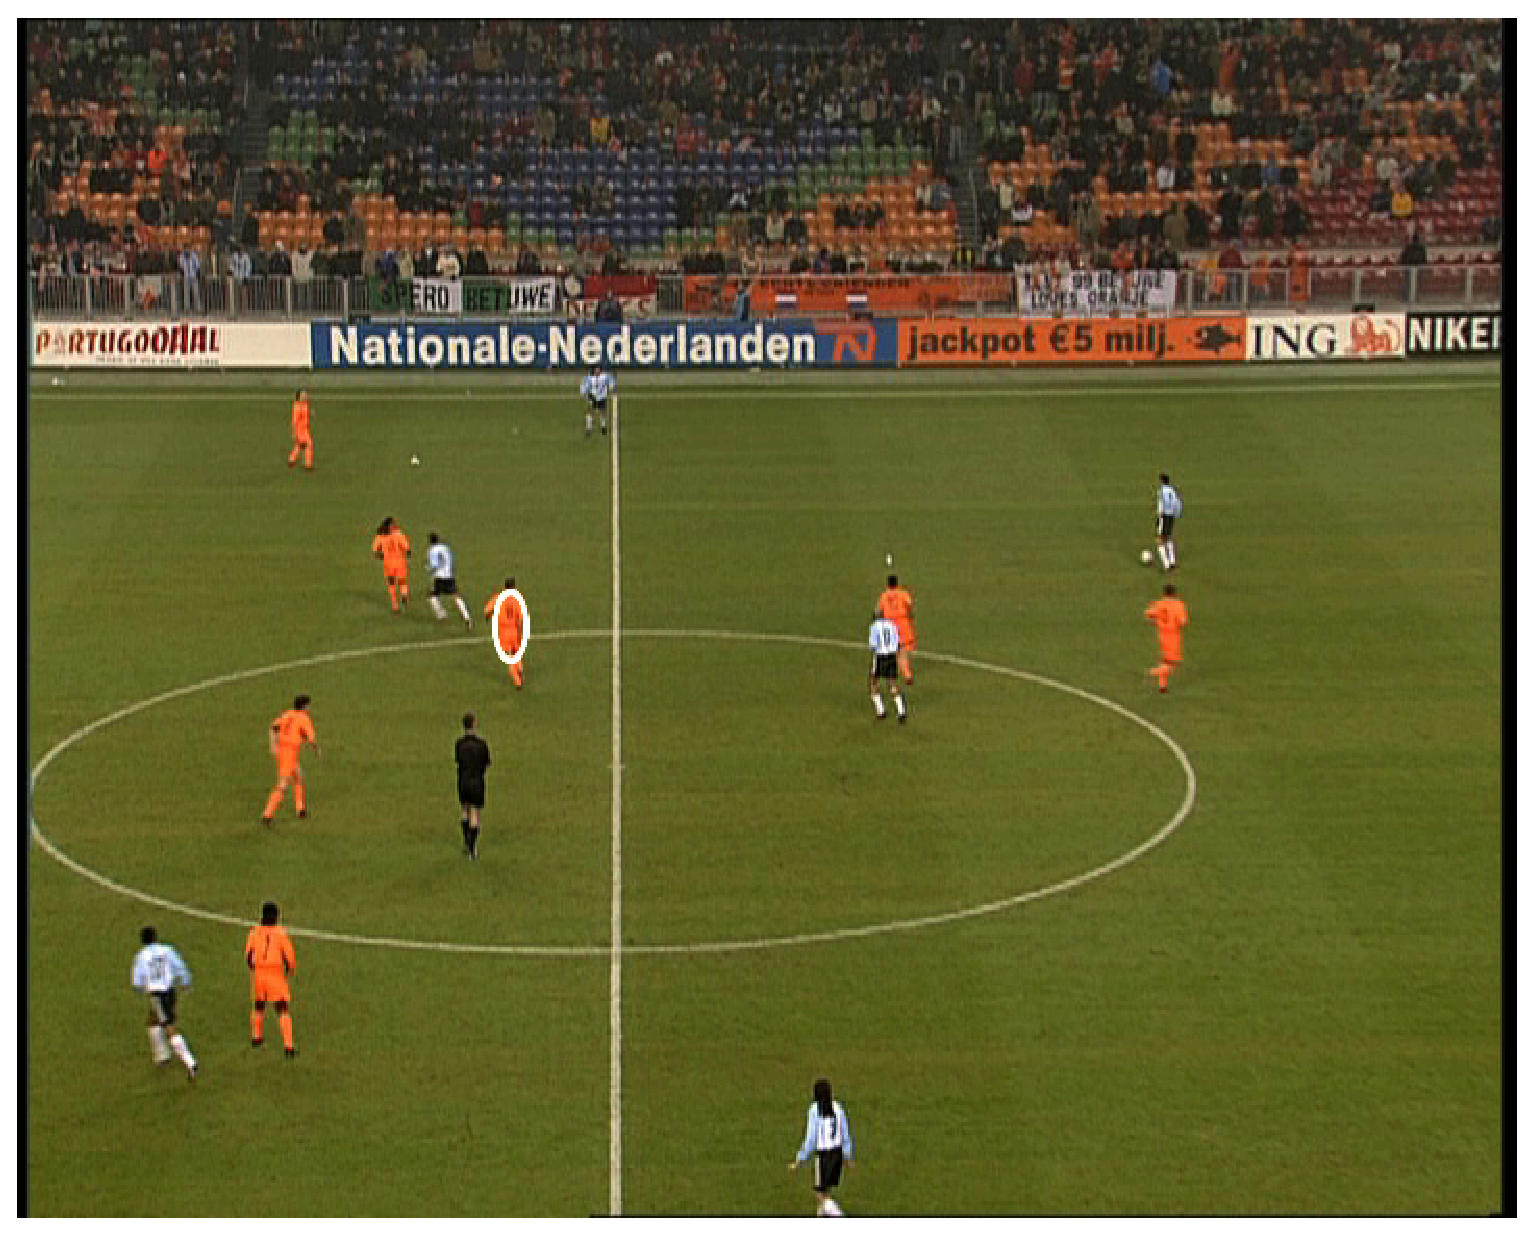
\includegraphics[height=5.0cm]{img/soccer_orange_scene}
\label{fig:1a}
}
\subfigure[The nature domain, a hunting cheetah.]{
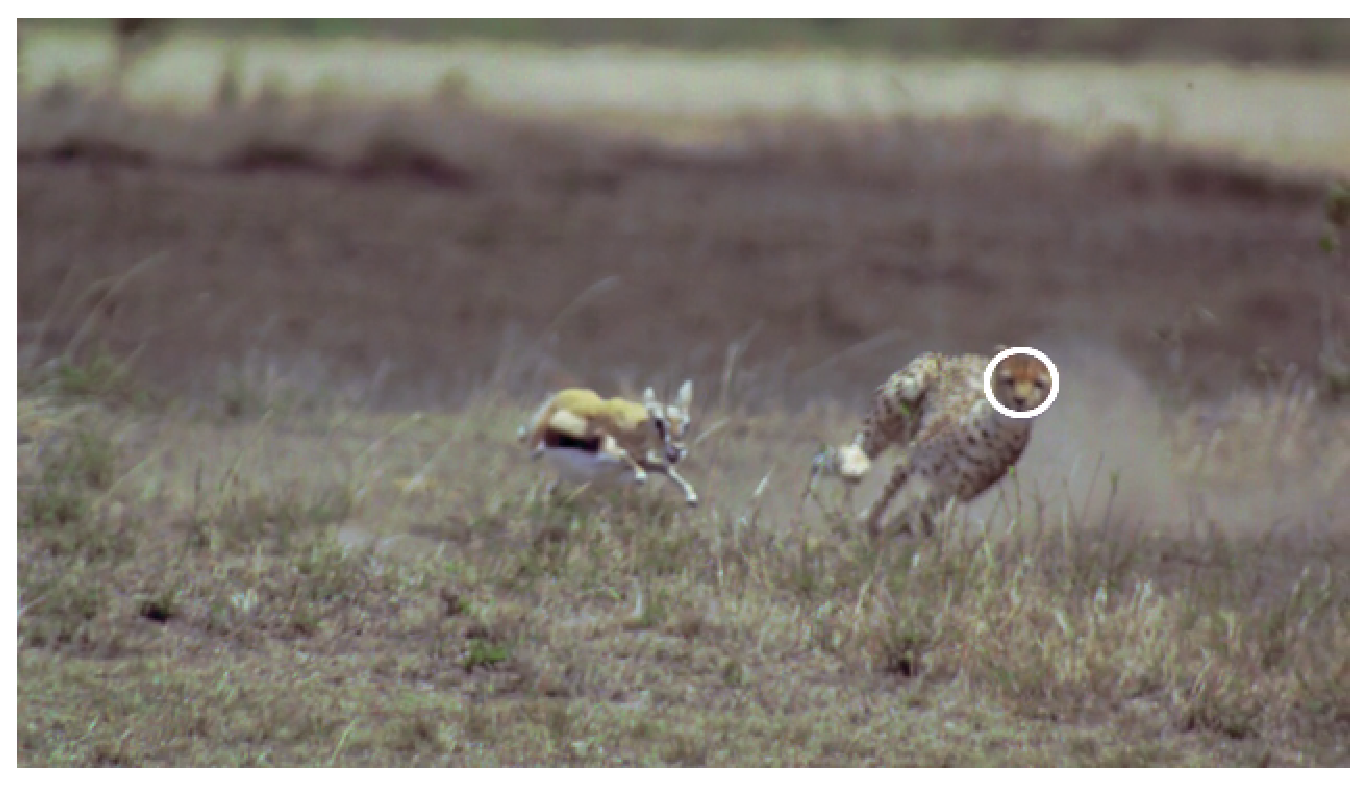
\includegraphics[height=5.0cm]{img/earth_cheetah_scene}
\label{fig:1b}
}
\caption{\ref{fig:1a} shows the sport domain where we track an orange soccer
player on the left. \ref{fig:1b} shows a scene from the movie Earth, where we
track the head of a cheetah chasing its prey.}
\label{fig:videos}
\end{figure}

\begin{algorithm}
	\caption{MeanShiftTracker($V$, $n$)}
	\begin{algorithmic}[1]
	\REQUIRE The video $V$ with $n$ frames
	\STATE $f_1 \leftarrow V[1]$ \COMMENT{Set the current frame}
	\STATE $\mathbf{y_0} \leftarrow \mathcal{S}(f_1)$ \COMMENT{Select target, store location}
	\STATE $\mathbf{q} \leftarrow \mathcal{M}(f_1, \mathbf{y_0})$ \COMMENT{Create the target model}
	\FOR{$i = 1$ to $n$}
		\STATE $f_i \leftarrow V[i]$
		\STATE $\mathbf{p_0} \leftarrow \mathcal{M}(f_i, \mathbf{y_0})$
		\STATE $bc_0 \leftarrow \mathcal{B}(\mathbf{p_0}, \mathbf{q})$ \COMMENT{Compute Bhattacharyya coefficient}
		\WHILE{true}
			\STATE $\mathbf{W} \leftarrow \mathcal{W}(f_i, \mathbf{y_0}, \mathbf{q}, \mathbf{p_0})$ \COMMENT{Compute the weights matrix}
			\STATE $\mathbf{y_1} \leftarrow \mathbf{y_0} + \mathcal{L}(\mathbf{W})$ \COMMENT{Compute the mean shift}
			\STATE $\mathbf{p_1} \leftarrow \mathcal{M}(f_i, \mathbf{y_1})$
			\STATE $bc_1 \leftarrow \mathcal{B}(\mathbf{p_1}, \mathbf{q})$
			\WHILE{$bc_1 < bc_0$} 
				\STATE $\mathbf{y_1} \leftarrow \frac{1}{2} \dot (\mathbf{y_0} + \mathbf{y_1})$ \COMMENT{Interpolate $\mathbf{y_1}$ if we shifted too far}
				\STATE $\mathbf{p_1} \leftarrow \mathcal{M}(f_i, \mathbf{y_1})$
				\STATE $bc_1 \leftarrow \mathcal{B}(\mathbf{p_1}, \mathbf{q})$
			\ENDWHILE
			\STATE $\mathbf{p_0} \leftarrow \mathbf{p_1}$
			\STATE $\mathbf{y_0} \leftarrow \mathbf{y_1}$
			\STATE $bc_0 \leftarrow bc_1$
			\IF{$\| \mathbf{y_1} - \mathbf{y_0} \| < \epsilon$}
				\STATE break \COMMENT{Break if locations are nearly equal}
			\ENDIF
		\ENDWHILE
	\ENDFOR
	\medskip
	\end{algorithmic}
\label{alg:mst}
\end{algorithm}

\section{Experiments and Results} \label{sec:results}
For our experiments we applied the tracker to videos within two different
domains, nature and sports. Figure \ref{fig:videos} shows the tracker in action
on both domains. In both videos a distinctive object was tracked using the various color models
and for each color model various histogram sizes, see Table \ref{tbl:bins}.

\begin{table}[!ht]
\centering
\begin{tabular}{c|c|c}
$N$   & $N^{1/2}$ & $N^{1/3}$\\\hline\hline
$2^6$ & $2^3$     & $2^2$\\\hline
$3^6$ & $3^3$     & $3^2$\\\hline
$4^6$ & $4^3$     & $4^2$\\\hline
$5^6$ & $5^3$     & $5^2$\\\hline
\end{tabular}
=
\begin{tabular}{r|r|r}
$N$     & $N^{1/2}$ & $N^{1/3}$\\\hline\hline
$64$    & $8$       & $4$\\\hline
$729$   & $27$      & $9$\\\hline
$4096$  & $64$      & $16$\\\hline
$15625$ & $125$     & $25$\\\hline
\end{tabular}
\caption{Histogram sizes (i.e. number of bins).}
\label{tbl:bins}
\end{table}

For a (somewhat) objective analysis of the various color models and various
histogram sizes, we chose to manually annotate the position of the target
objects within the frame sequences of each video. In figures \ref{fig:soccer}
and \ref{fig:cheetah} we compared the performance of
the five different color models for four different numbers of bins on the soccer
movie when tracking the orange player and cheetah movie when tracking the
cheetahs head respectively.

Both figures show our final results displayed in
four graphs with frame numbers on the $x$-axis and the Euclidean distance,
between the trackers output and our labeled data, on the $y$-axis. All graphs
show a very distinctive pattern on the color models that lost track. In the
sports domain (figure \ref{fig:soccer}) this is the result of occlusion caused by
a white player. The white player walks in front of the orange player (the
target object) and pushes the model away at which point it finds a new orange
player and starts tracking him. In the nature domain (figure \ref{fig:cheetah})
if the tracker gets lost this means that some portion of the background is
classified as the target object and the tracker starts tracking that region
instead.\\

The mean Euclidean error between the tracked target object and the ground truth
we annotated by hand is shown in table \ref{tbl:error}. Using the normalized
$rgb$ color space results in the highest accuracy for all our test cases.
This indicates that the $rgb$ color model is a robust one and would indeed be
our choice for object tracking. However we should note that running tests in two
domains might not be sufficient to determine the significance of these results.

\begin{table}[!ht]
\centering
\begin{tabular}{r||r|r|r|r|r}
	\emph{bins} & $RGB$ & $rgb$ & $HSV$ & $XYZ$ & $xyz$ \\ \hline \hline
	         64 &  51.8 &   6.8 &   8.1 & 114.2 &  81.3 \\ \hline
	        729 &  57.9 &   5.7 &   5.7 &  45.8 &  66.5 \\ \hline
	       4096 &  31.5 &   4.8 &  56.8 &  58.4 &   5.5 \\ \hline
	      15625 &  44.8 &   4.4 &   4.5 &  57.9 &   4.1 \\ \hline
\end{tabular}
\caption{Mean Euclidean error derived from 201 frames from the sports domain and
300 frames from the nature domain.}
\label{tbl:error}
\end{table}

\begin{figure}[!ht]
\centering
\subfigure[$64$ bins]{
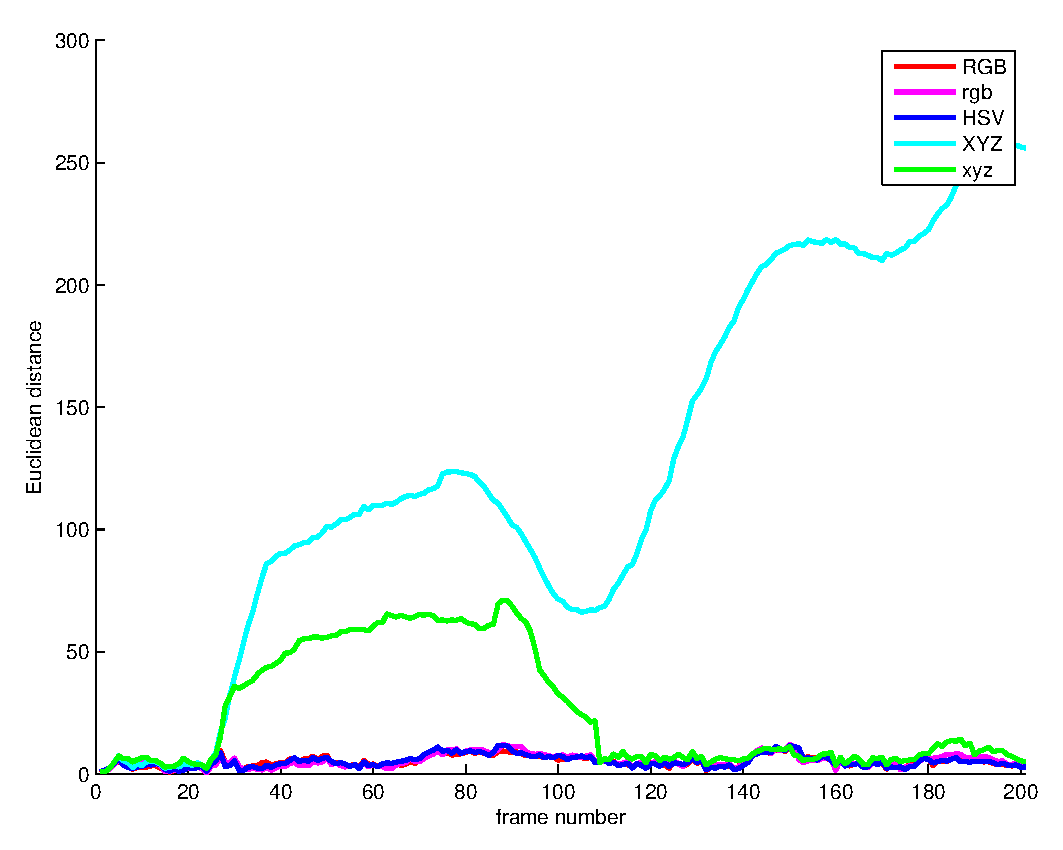
\includegraphics[height=6.0cm]{img/soccer_orange_64}
\label{fig:3a}
}
\subfigure[$729$ bins]{
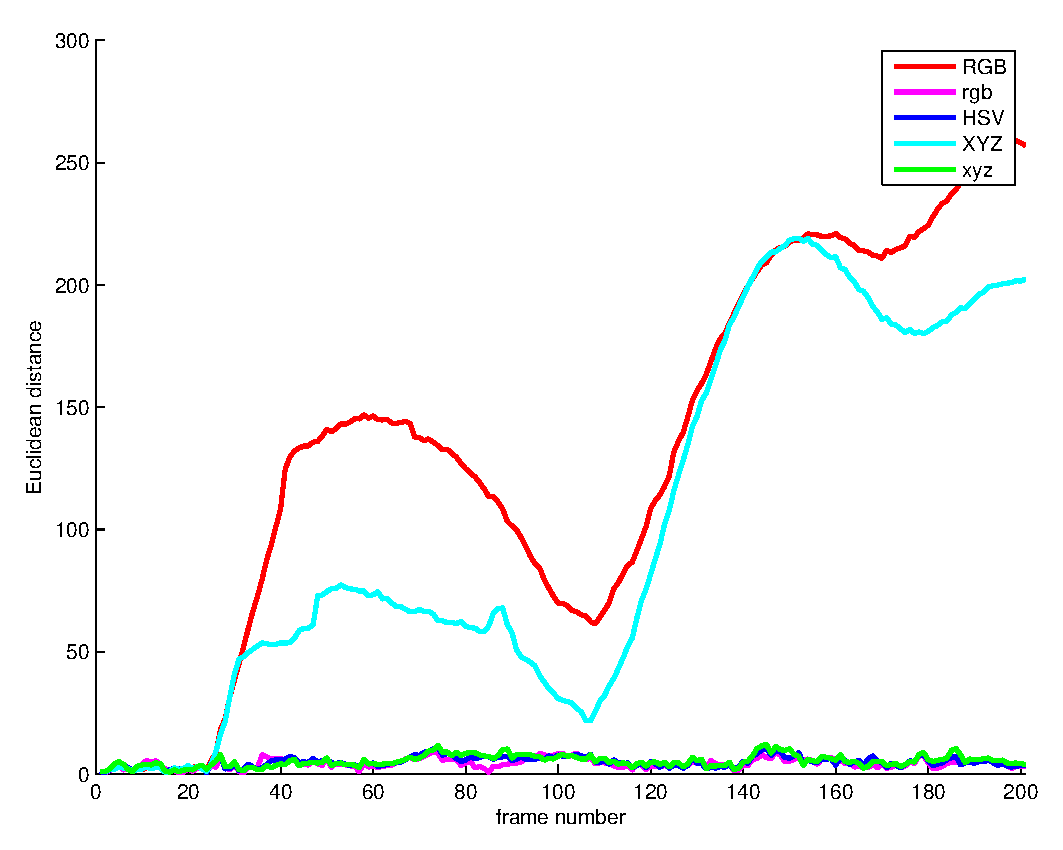
\includegraphics[height=6.0cm]{img/soccer_orange_729}
\label{fig:3b}
}
\\
\subfigure[$4096$ bins]{
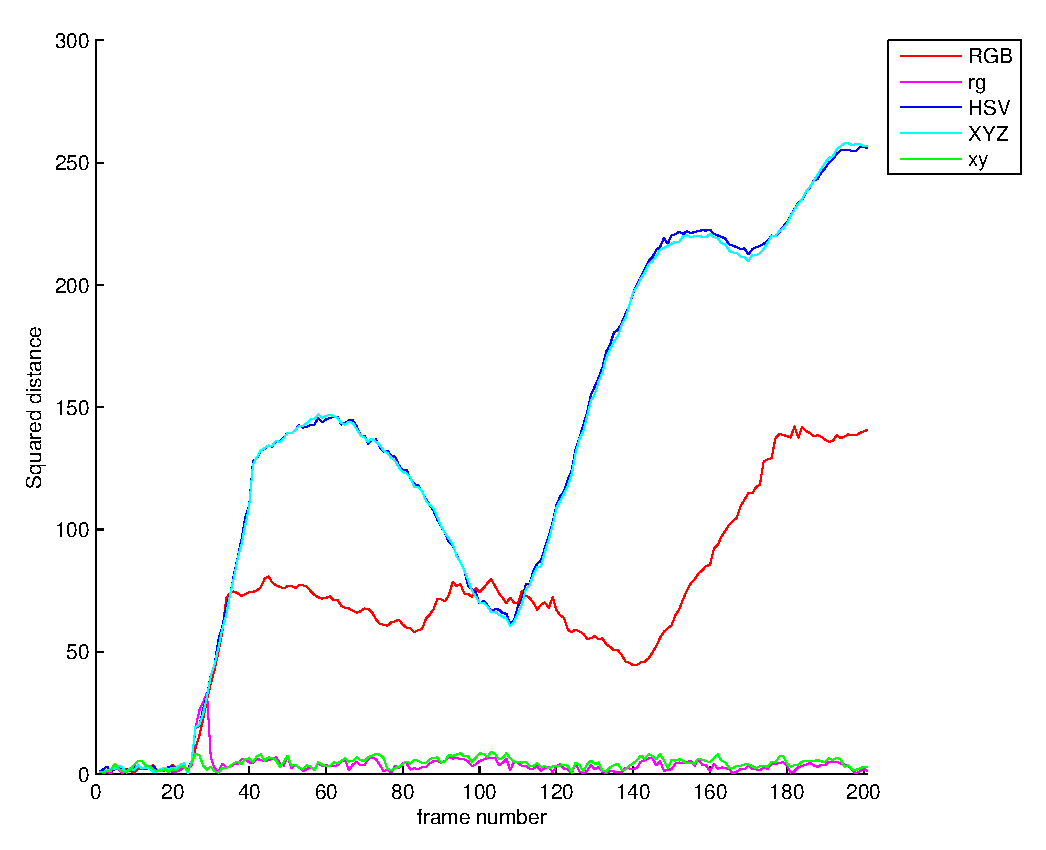
\includegraphics[height=6.0cm]{img/soccer_orange_4096}
\label{fig:3c}
}
\subfigure[$15625$ bins]{
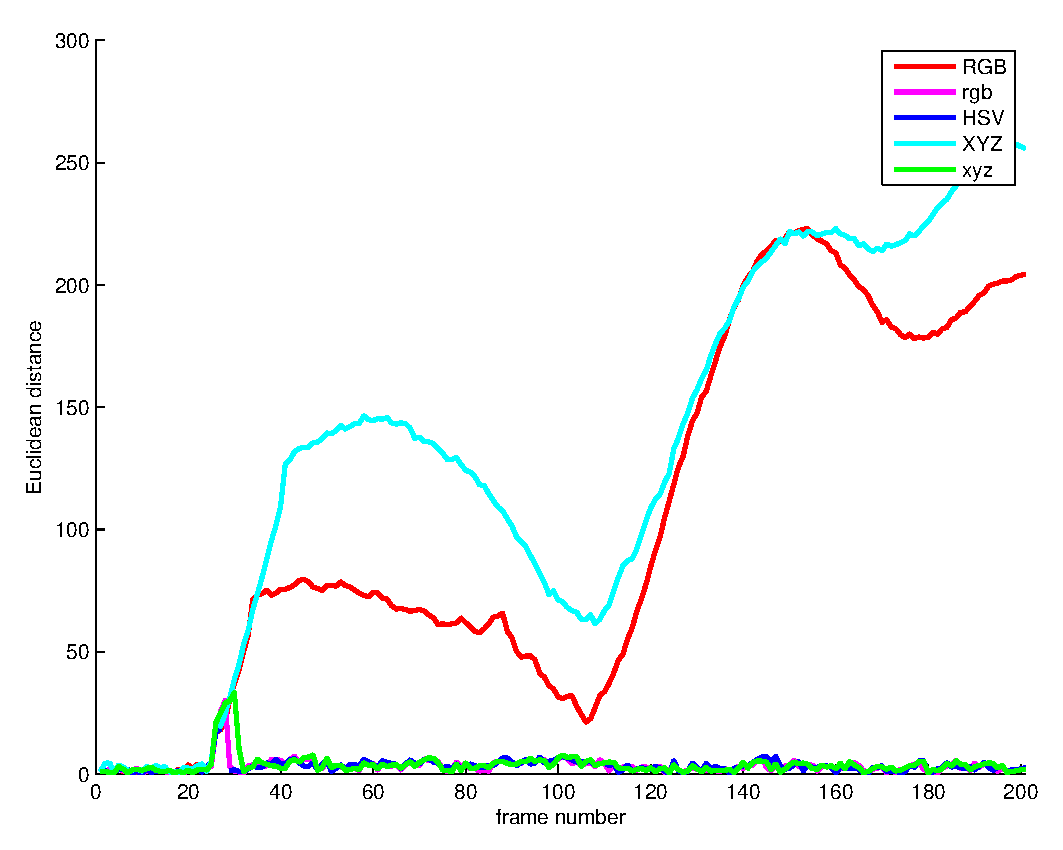
\includegraphics[height=6.0cm]{img/soccer_orange_15625}
\label{fig:3d}
}
\caption{Each graph shows the performance of the five different color models
for a number of bins on the soccer movie when tracking the orange player. All
four graphs show a very distinctive pattern on the color models that lost
track.}
\label{fig:soccer}
\end{figure}

Figure \ref{fig:2a} shows that several color models have completely lost track,
indicating that $64$ bins is not enough. In \ref{fig:2b} only the $xyz$ model failed.
In both \ref{fig:2c} and \ref{fig:2d} all color models show good performance.
This indicates that the more bins used, the better the model becomes.

\begin{figure}[!ht]
\centering
\subfigure[$64$ bins]{
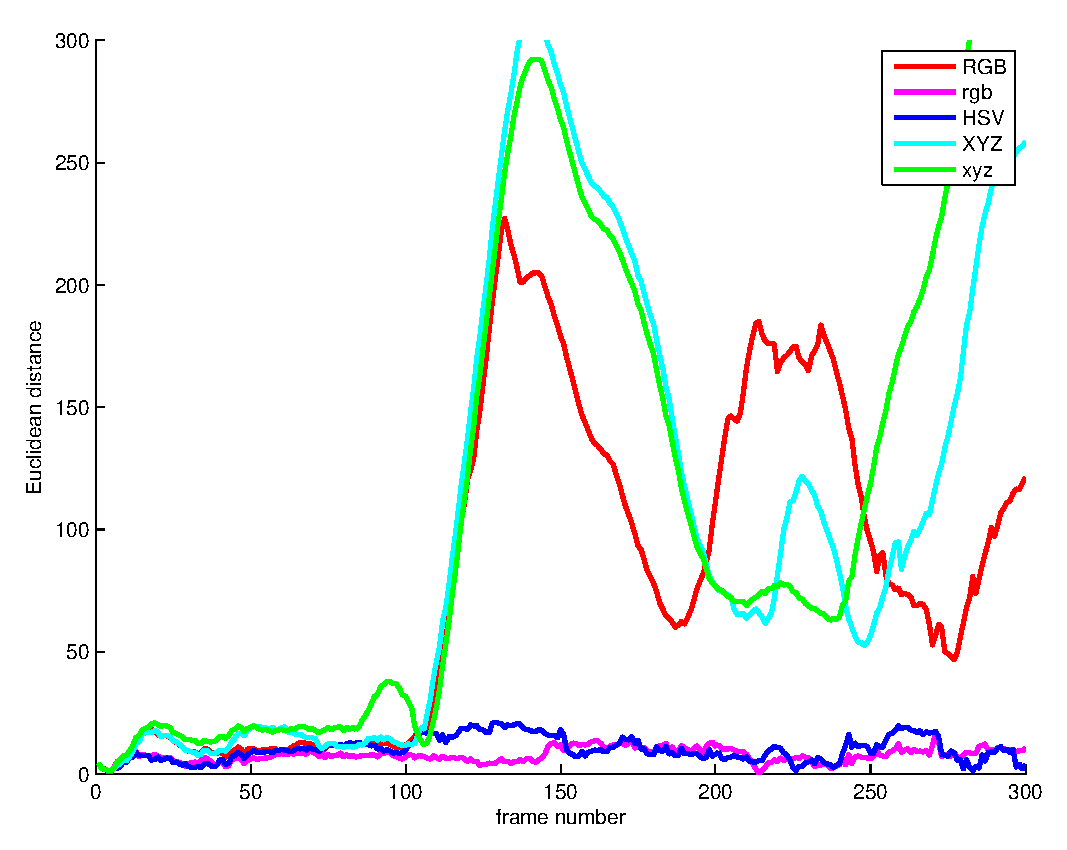
\includegraphics[height=6.0cm]{img/earth_cheetah_64}
\label{fig:2a}
}
\subfigure[$729$ bins]{
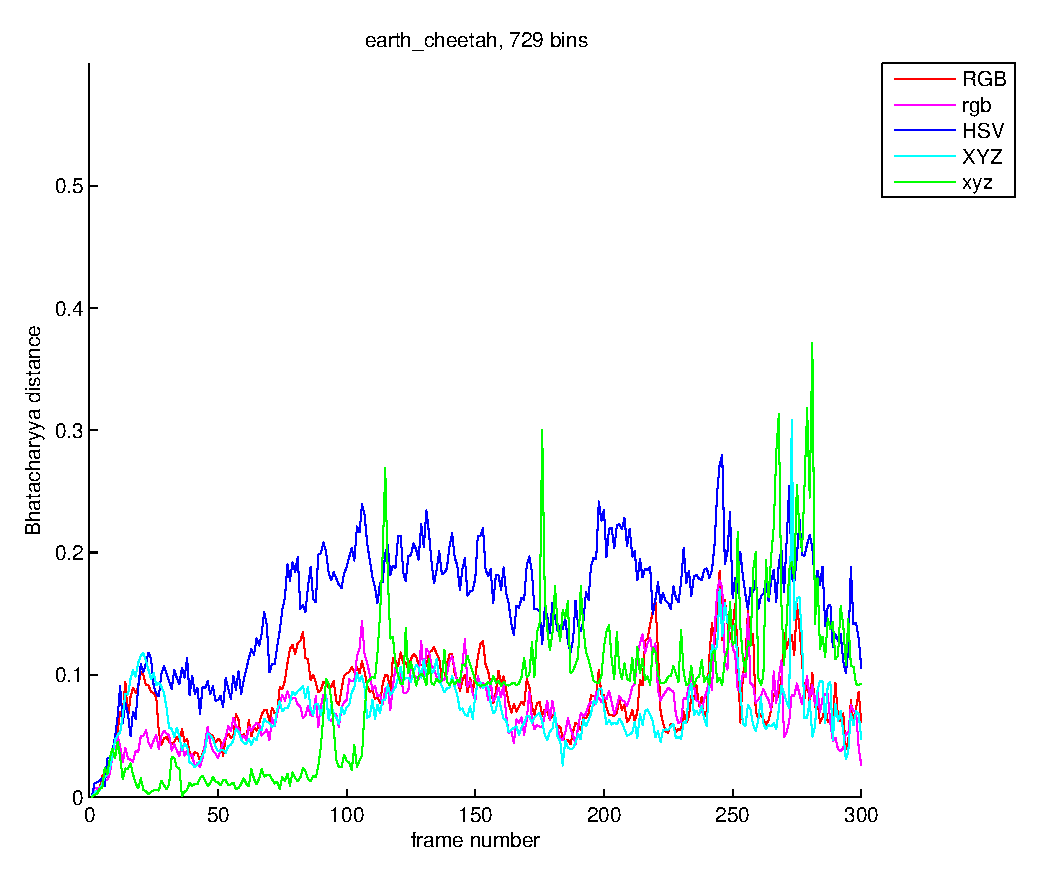
\includegraphics[height=6.0cm]{img/earth_cheetah_729}
\label{fig:2b}
}
\\
\subfigure[$4096$ bins]{
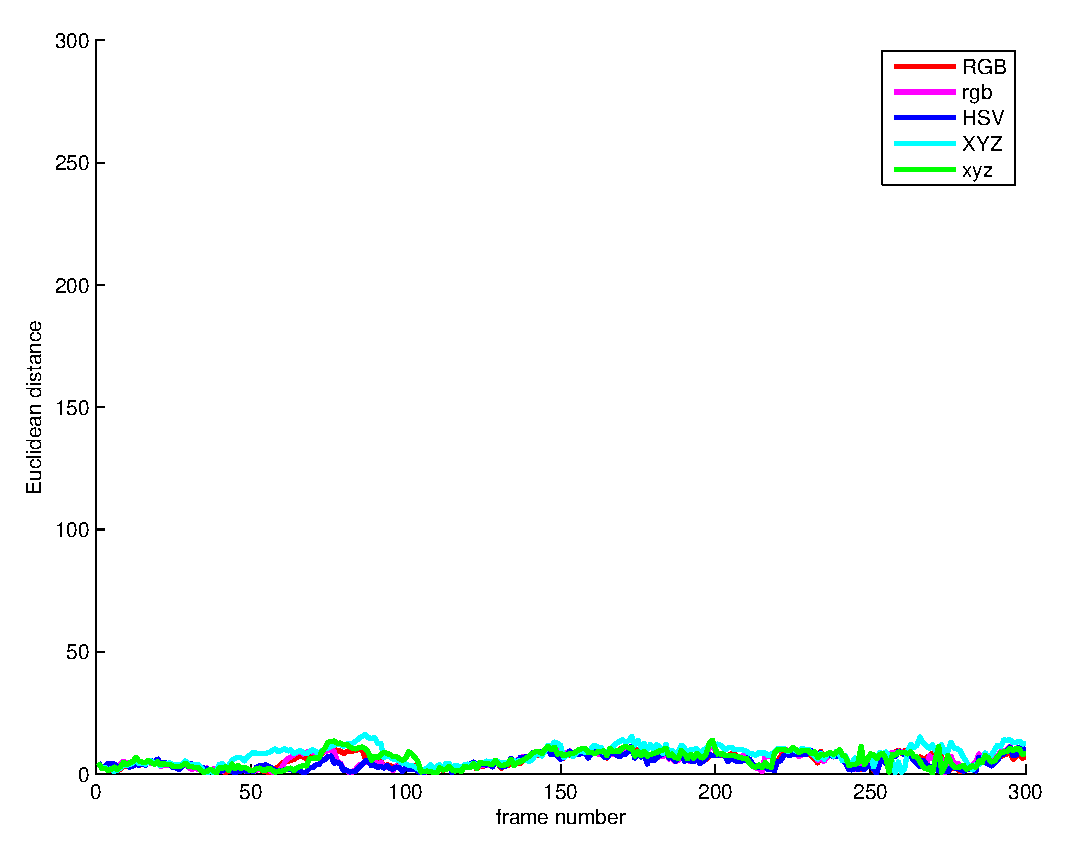
\includegraphics[height=6.0cm]{img/earth_cheetah_4096}
\label{fig:2c}
}
\subfigure[$15625$ bins]{
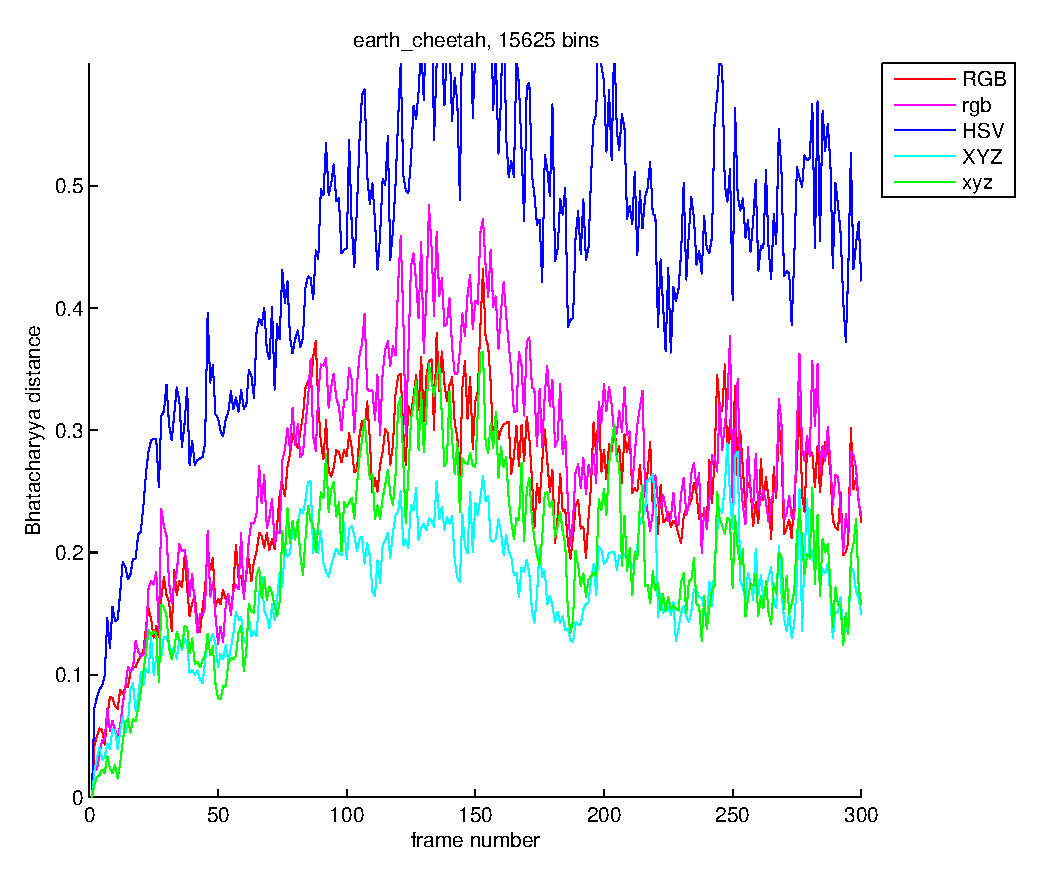
\includegraphics[height=6.0cm]{img/earth_cheetah_15625}
\label{fig:2d}
}
\caption{Each graph shows the performance of the five different color models for
a number of bins on the cheetah movie when tracking the cheetahs head.
\ref{fig:2a} shows that several color models have completely lost track. In
\ref{fig:2b} only the $xyz$ model failed. In both \ref{fig:2c} and \ref{fig:2d}
all color models show good performance.}
\label{fig:cheetah}
\end{figure}

\section{Conclusions} \label{sec:conclusion}
This report introduced an implementation of the mean shift tracking algorithm,
comparing its performance using various color models applied to videos from two
different domains.  From the results we conclude that a significant histogram
size should be chosen to represent a model for robust tracking. An insufficient
amount of bins over generalizes the model, at which point the tracker loses its
target object as both the target and background are (according to the model)
indistinguishable.  Furthermore, the best color model, according to our
results, is the normalized $rgb$ model. That is, the $rgb$ color model had the
best overall performance across the domains and various histogram sizes.
Although the mean shift tracker is indeed robust, it does have its limitations.
It has difficulty handling occlusions, and when two similar objects overlap it
can jump to the other object.

\section{Future Work} \label{sec:future}
A lot can be improved in the current implementation. We will discuss some of
these improvements in this section.

\paragraph{Scale Invariance} The current implementation is not scale invariant. This
results in tracking problems when an object is getting closer or further away
from the camera or when a camera zooms in or out. In these cases the target
model gets outdated and the eventually the tracker will fail. Implementing
scale invariance will solve this problem. This can be done by computing the
Epanechnikov kernel for various scales and select the best scale for each
frame using the Bhattacharyya distance.

\paragraph{Kalman Filter} When the target object gets occluded by another object
or some other part of the scene the tracker might lose the target object. In
general the tracker tends to jitter a lot while tracking the target object.
It's likely that applying a Kalman Filter will solve both these problems. By
doing so, an assumption about the expected motion (i.e. the expected location
of the target object in the next frame) is made and therefore the tracker would
become much more stable.

\paragraph{Color Space} The tracker assumes a color model has a priori been
chosen. We suspect that the best choice for a color model depends on the domain
or the scene. It might be a good idea to implement some automated analysis to
determine which color space is best suited for the target model for every
individual scene. For example the color space model with the highest variance
could be chosen or the color model in which the target object differs most from
the rest of the scene.

\paragraph{Spatial Layout} To improve the target model (especially when complex
target objects have to be tracked) one could divide the kernel into several
tiles to store some information about the spatial layout of the target object
to create more discriminative models. One should use caution with respect to
the problem of over fitting.

\renewcommand\bibname{References}
\bibliography{references}
\bibliographystyle{IEEEtran}
\end{document}
